\documentclass[acmnow]{acmtrans2m}


\usepackage{graphicx}


\newtheorem{theorem}{Theorem}[section]
\newtheorem{conjecture}[theorem]{Conjecture}
\newtheorem{corollary}[theorem]{Corollary}
\newtheorem{proposition}[theorem]{Proposition}
\newtheorem{lemma}[theorem]{Lemma}
\newdef{definition}[theorem]{Definition}
\newdef{remark}[theorem]{Remark}


           
\markboth{Nigel Stanger}{...}

\title{Scalability of Techniques for Online Geovisualization of Web Site Hits}
            
\author{NIGEL STANGER \\ University of Otago}
            
\begin{abstract} 
A useful approach to visualizing the geographical distribution of web
site hits is to geolocate the IP addresses of hits and plot them on a
world map. This can be achieved by dynamic generation and display of map
images at the server and/or the client. This paper compares the
scalability with respect to source data size of four techniques for
dynamic map generation and display: generating a single composite map
image, overlaying transparent images on an underlying base map,
overlaying CSS-enabled HTML on an underlying base map and generating a
map using Google Maps. These four techniques embody a mixture of
different display technologies and distribution styles. The results show
that all four techniques are suitable for small data sets, but that the
latter two techniques scale poorly to larger data sets.
\end{abstract}
            
\category{C.4}{Performance of Systems}{Performance attributes}
\category{C.2.4}{Computer-Communication Networks}{Distributed Systems}[distributed applications]
\category{H.3.5}{Information Storage and Retrieval}{Online Information Services}[web-based services]
            
\terms{Experimentation, Measurement, Performance} 
            
\keywords{downloads, geolocation, geovisualization, scalability, Google
	Maps, distribution style, dynamic map generation}
            
\begin{document}


\bibliographystyle{acmtrans}

            
\begin{bottomstuff} 
Author's address: N. Stanger, Department of Information Science,
University of Otago, PO Box 56, Dunedin 9054, New Zealand.
\end{bottomstuff}
            
\maketitle


\section{Introduction}
\label{sec-introduction}

When administering a web site, it is quite reasonable to want
information on the nature of traffic to the site. Information on the
geographic sources of traffic can be particularly useful in the right
context. For example, an e-commerce site might wish to determine the
geographical distribution of visitors to the site, so as to decide where
best to target marketing resources. One approach to doing so is to plot
geographical locations on a map. Geographical information systems (GIS)
were already being used for these kinds of purposes prior to the advent
of the World Wide Web \cite{Beau-JR-1991-GIS}, and it is a natural
extension to apply these ideas to online visualization of web site hits.

The author's interest in this area derives from implementing a pilot
digital institutional repository for the University of Otago School of
Business\footnote{\url{http://eprints.otago.ac.nz/}} in November 2005
\cite{Stan-N-2006-running}, using the GNU
EPrints\footnote{\url{http://www.eprints.org/}} repository management
software. This repository quickly attracted interest from around the
world and the number of abstract views and document downloads began to
steadily increase. There was great interest within the University in
tracking this increase, particularly with respect to where in the world
the hits were coming from. The EPrints statistics management software
developed at the University of Tasmania \cite{Sale-A-2006-stats} proved
very useful in this regard, providing detailed per-eprint and
per-country download statistics; an example of the latter is shown in
Figure~\ref{fig-tas-stats}. However, while this display provides an
ordered ranking of the number of hits from each country, it does not
provide any greater detail beyond the country level, nor does it provide
any visual clues as to the spatial distribution of hit sources around
the globe.


\begin{figure}
	\centering
	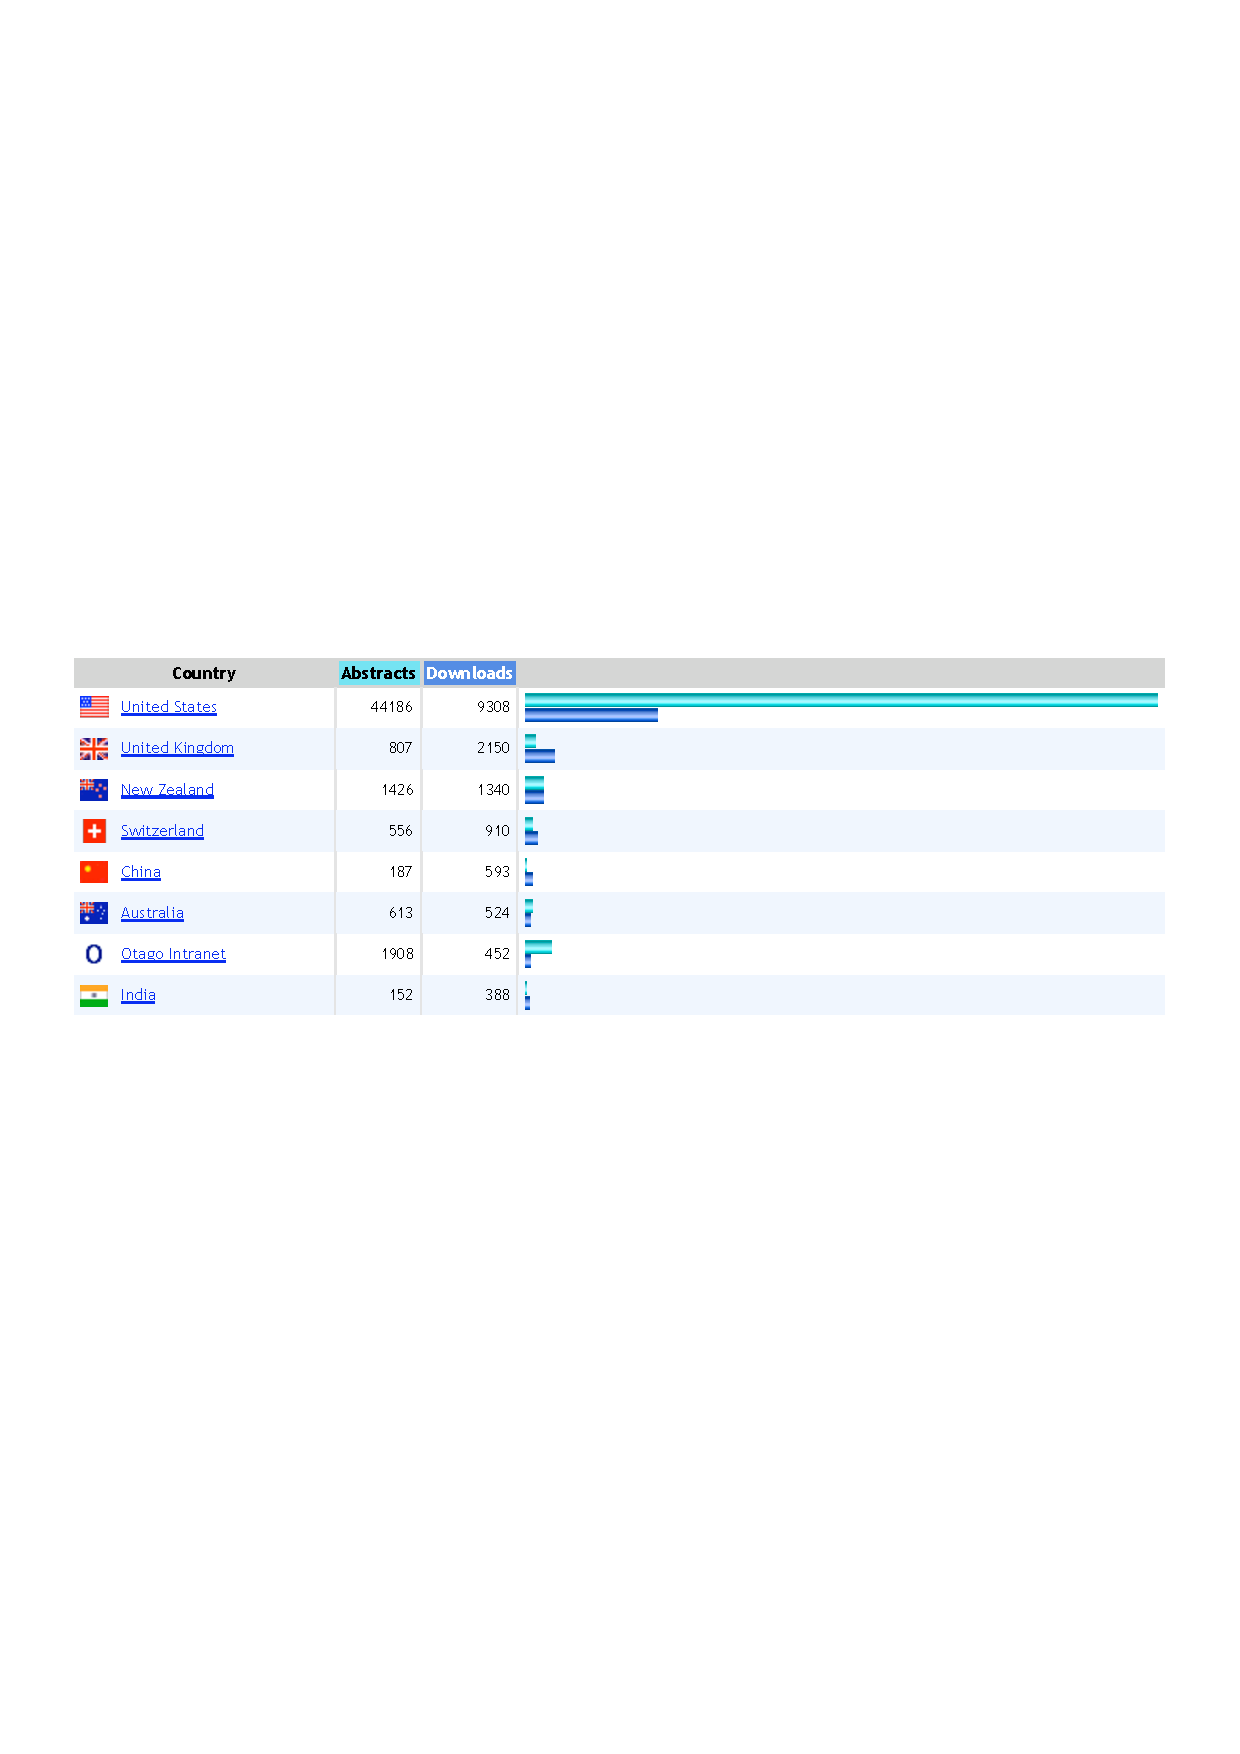
\includegraphics[width=\textwidth,keepaspectratio]{tasmania_stats}
	\caption{A portion of the by-country display for the Otago EPrints
	repository, generated by the Tasmania statistics software
	\protect\cite{Sale-A-2006-stats}.}
	\label{fig-tas-stats}
\end{figure}


The author therefore began to explore possible techniques for plotting
repository hit data onto a world map, with the aim of adding this
capability to the Tasmania statistics package. Preference was given to
techniques that could be used within a modern web browser without the
need to manually install additional client software, so as to make the
new feature available to the widest possible audience and reduce the
impact of wide variation in client hardware and software environments
\cite[pp.\ 27--28]{Offu-J-2002-quality}.

There have been several prior efforts to geovisualize web activity.
\citeN{Lamm-SE-1996-webvis} developed a sophisticated system for
real-time visualization of web traffic on a 3D globe, but this was
intended for use within a virtual reality environment, thus limiting its
general applicability. \citeN{Papa-N-1998-Palantir} described a similar
system called \emph{Palantir}, which was written as a Java applet and
thus able to be run within a web browser, assuming that a Java virtual
machine was available. \citeN[pp.\ 100--103]{Dodg-M-2001-cybermap}
describe these and several other related systems for mapping Web and
Internet traffic.

These early systems suffered from a distinct limitation in that there
was no public infrastructure in place for geolocating IP addresses (that
is, translating them into latitude/longitude coordinates). They
generally used \texttt{whois} lookups or parsed the domain name in an
attempt to guess the country of origin, with fairly crude results
\cite{Lamm-SE-1996-webvis}. Locations outside the United States were
typically aggregated by country and mapped to the capital city
\cite{Lamm-SE-1996-webvis,Papa-N-1998-Palantir,Jian-B-2000-cybermap}.
Reasonably accurate and detailed databases were commercially available
at the time \cite[p.\ 1466]{Lamm-SE-1996-webvis}, but were not generally
available to the public at large, thus limiting their utility.

The situation has improved considerably in the last five years, however,
with the advent of freely available and reasonably accurate geolocation
services\footnote{Such as \url{http://www.maxmind.com/} or
\url{http://www.ip2location.com/}.} with worldwide coverage and
city-level resolution. For example, Maxmind's \emph{GeoLite City}
database is freely available and claims to provide ``60\% accuracy on a
city level for the US within a 25 mile radius''
\cite{Maxm-G-2006-GeoLiteCity}. Their commercial \emph{GeoIP City}
database claims 80\% accuracy for the same parameters.

The techniques used by these prior systems can generally be divided into
two classes. The first class of techniques generate a single bitmap
image that contains both the map and the graphics representing web hits.
This can be achieved by programmatically plotting points onto a base map
image; the composite image is then displayed at the client. This class
of techniques shall henceforth be referred to as \emph{single-layer}
techniques. The second class of techniques separately return both a base
map image and some kind of overlay containing the plotted points. The
overlay and the base map are then displayed as separate items at the
client. This class of techniques shall henceforth be referred to as
\emph{multi-layer} techniques.

Both classes of techniques have been used in the aforementioned systems,
but multi-layer techniques appear to have been the most prevalent. For
example, Palantir used a multi-layer technique, in which a Java applet
running at the client overlaid graphic elements onto a base map image
retrieved from the now-defunct Xerox online map server
\cite{Papa-N-1998-Palantir}. A more recent example is the Google Maps
API \cite{Goog-M-2006-maps}, which enables web developers to easily
embed interactive maps within web pages. Google Maps is a dynamic
multi-layer technique that has only become feasible relatively recently
with the advent of widespread support for CSS positioning and Ajax
technologies \cite{Garr-JJ-2005-Ajax} in many browsers.

Multi-layer techniques enjoy a particular advantage over single-layer
techniques, in that they provide the potential for a more flexible
GIS-like interaction with the map, with multiple layers that can be
activated and deactivated as desired. This flexibility could explain why
such techniques appear more prevalent in the literature. As will be seen
shortly, however, web-based multi-layer techniques tend to rely either
on the installation of additional client-side software, or on more
recent web technologies such as CSS and Ajax. Single-layer techniques,
in contrast, typically do not rely on these things. Single-layer
techniques should therefore be portable to a wider range of client and
server environments.

Each map generation and display technique comprises a specific
technology or collection of technologies (such as transparent bitmap
overlays + CSS positioning), implemented using a specific distribution
style. For example, a particular single-layer technique might be
implemented completely server-side while another might use a mixture of
server-side and client-side processing. Similarly, multi-layer
techniques may adopt different distribution styles, and the overlays
themselves might take the form of transparent images, absolutely
positioned HTML elements, dynamically generated graphics, etc.

Given the wide variety of possible techniques that were available, the
next question was which techniques would be most suitable? Ideally, a
technique should not only efficiently fulfil the task of plotting
repository hits on a map, but also provide tangible benefits to
end-users. Scalability is a key issue for web applications in general
\cite[p.\ 28]{Offu-J-2002-quality}, and for online activity
visualization in particular \cite[p.\ 50]{Eick-SG-2001-sitevis}, so
techniques that could scale to a large number of points were of
particular interest. For example, at the time of writing the Otago
EPrints repository had been accessed from 13,000 distinct IP addresses,
each potentially representing a distinct geographical location.
Separating out the type of hit (abstract view versus document download)
increased that figure to nearly 16,000. Informal testing with these data
suggested that a single-layer composite map image would perform well
with this volume of data, taking at most a few seconds to load and
display. Conversely, it appeared that Google Maps would not perform
well, taking on the order of minutes to load and display a map
containing a few thousand points.

The range of techniques was first narrowed down to just four
(server-side image generation, server-side image overlay, server-side
HTML overlay and Google Maps); the selection process and details of the
techniques chosen are discussed in Section~\ref{sec-techniques}. The
scalability of these four techniques was then tested to determine how
well each technique handled large numbers of points. A series of
experiments was conducted on each technique with progressively larger
synthetic data sets, and the data set volume, elapsed time and memory
usage were measured. The experimental design is discussed in
Section~\ref{sec-experiment}.

Informal tests suggested that the server-side image generation and the
server-side image overlay techniques would scale best, and this was
borne out by the results of the experiments, which show that both
techniques scale reasonably well to very large numbers of points. The
other two techniques proved to be reasonable for relatively small
numbers of points (generally less than about 500--1,000), but their
performance deteriorated rapidly beyond this. The results are discussed
in more detail in Section~\ref{sec-results}.

It should be noted that the intent of the experiments was not to
identify statistically significant differences in performance across the
four techniques. It was expected that variations across techniques would
be reasonably clear-cut, and the experiments were designed to test this
expectation. However, the two best performing techniques, server-side
image generation and server-side image overlay, produced very similar
results, so a more formal statistical analysis of these techniques may
be warranted. This and other possible future directions are discussed in
Section~\ref{sec-conclusion}.


\section{Technique selection}
\label{sec-techniques}

In this section the four techniques that were chosen for testing are
discussed in more detail, along with the reasons for choosing these
particular techniques. First, the impact of distribution style on the
choice of technique is discussed. This is followed by an examination of
how each technique works in practice, its implementation requirements,
its relative advantages and disadvantages, and any other issues peculiar
to the technique.


\subsection{Distribution style}
\label{sec-distribution}

\citeN{Wood-J-1996-vis} and \citeN{MacE-AM-1998-GIS} identified four
distribution styles for web-based geographic visualization software. The
\emph{data server} style is where the server only supplies raw data, and
all manipulation, display and analysis takes place at the client. In
other words, this is primarily a client-side processing model, as
illustrated in Figure~\ref{fig-distribution-styles}(a). For example,
Palantir implemented a multi-layer technique using this distribution
style \cite{Papa-N-1998-Palantir}, where the source data were generated
at the server and the map was generated, displayed and manipulated by a
Java applet running at the client. The data server distribution style
can provide a very dynamic and interactive environment to the end user,
but clearly requires support for executing application code within the
web browser, typically using something like JavaScript, Java applets or
Flash. JavaScript is now tightly integrated into most browsers, but the
same cannot be said for either Java or Flash. That is, the existence of
a Java virtual machine or Flash plugin cannot necessarily be guaranteed
in every browser, which violates the requirement to avoid manual
installation of additional client-side software. Java- or Flash-based
data server techniques can therefore be eliminated from consideration,
but JavaScript-based data server techniques are feasible. Indeed, Google
Maps is an example of such a technique (see Section~\ref{sec-overlay}).


\begin{figure}
	\centering
	\begin{tabular}{ccc}
		\includegraphics[scale=0.9]{data_server}	&
		\qquad	&
		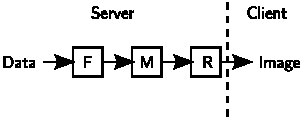
\includegraphics[scale=0.9]{image_server}	\\
		\footnotesize (a) Data server	&
		\qquad	&
		\footnotesize (b) Image server	\\
		\\
		\\
		\includegraphics[scale=0.9]{model_interaction}	&
		\qquad	&
		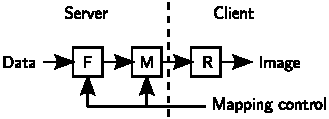
\includegraphics[scale=0.9]{shared}	\\
		\footnotesize (c) Model interaction environment	&
		\qquad	&
		\footnotesize (d) Shared environment	\\
	\end{tabular}
	\caption{Distribution styles for web-based geographic visualization
	\protect\cite{Wood-J-1996-vis}. (F = filtering, M = mapping, R =
	rendering.)}
	\label{fig-distribution-styles}
\end{figure}


Conversely, the \emph{image server} style is where the display is
created and manipulated entirely at the server and is only passively
viewed at the client. In other words, this is primarily a server-side
processing model, as illustrated in
Figure~\ref{fig-distribution-styles}(b). Consequently, techniques that
use this style require no additional client-side software. The downside
is that the resultant visualization can tend to be very static and
non-interactive in nature, as it is typically just a simple bitmap
image.

The \emph{model interaction environment} style is where a model created
at the server can be explored at the client, as illustrated in
Figure~\ref{fig-distribution-styles}(c). \citeN{MacE-AM-1998-GIS} calls
this the ``3D model interaction'' style, but this seems slightly out of
place in the current context. \citeN{Wood-J-1996-vis} originally
intended this distribution style to apply to VRML models for GIS
applications, but it could be equally applied to any situation where an
interactive model is generated at the server, then downloaded to and
manipulated at the client. This is very similar to what happens with
many Flash-based applications, for example. ``Model interaction
environment'' therefore seems a more appropriate name for this style.
The key distinguishing feature of this style is that there is no further
interaction between the client and server after the model has been
downloaded. This means that while the downloaded model can be very
dynamic and interactive, changing the underlying data requires a new
model to be generated at the server and downloaded to the client.
Similar restrictions apply to techniques using this style as to the data
server style, so Java- and Flash-based model interaction environment
techniques can be eliminated from consideration. For similar reasons,
solutions such as VRML or SVG that require external browser plugins can
also be eliminated (although native support for SVG is beginning to
appear in some browsers). It may be possible to implement this
distribution style using only client-side JavaScript, but it is
presently unclear as to how effective this might be.

Finally, the \emph{shared environment} style is where data manipulation
is done at the server, but control of that manipulation, and rendering
and display all occur at the client, as illustrated in
Figure~\ref{fig-distribution-styles}(d). This is similar to the model
interaction environment style, but with the addition of a feedback loop
from the client to the server, thus enabling a more flexible and dynamic
interaction. Ajax technologies can easily support this kind of
distribution style. For example, \citeN{Saya-A-2006-GISWS} use Ajax to
integrate Google Maps with existing GIS visualization web services.
Specific shared environment techniques can be eliminated from
consideration based on the same criteria as were applied to the other
three styles (e.g., no Java- or Flash-based techniques).


\subsection{Single-layer techniques}
\label{sec-image-gen}

As noted earlier, single-layer techniques work by directly plotting
geolocated IP addresses onto a base map image, then displaying the
composite image at the client. A typical example of the kind of output
that might be produced is shown in Figure~\ref{fig-image}. Such
techniques require two specific components: software to programmatically
create and manipulate bitmap images (for example, the GD image
library\footnote{\url{http://www.boutell.com/gd/}}); and software to
transform latitude/longitude coordinates into projected map coordinates
on the base map (for example, the PROJ.4 cartographic projections
library\footnote{\url{http://www.remotesensing.org/proj/}}).


\begin{figure}
	\centering
	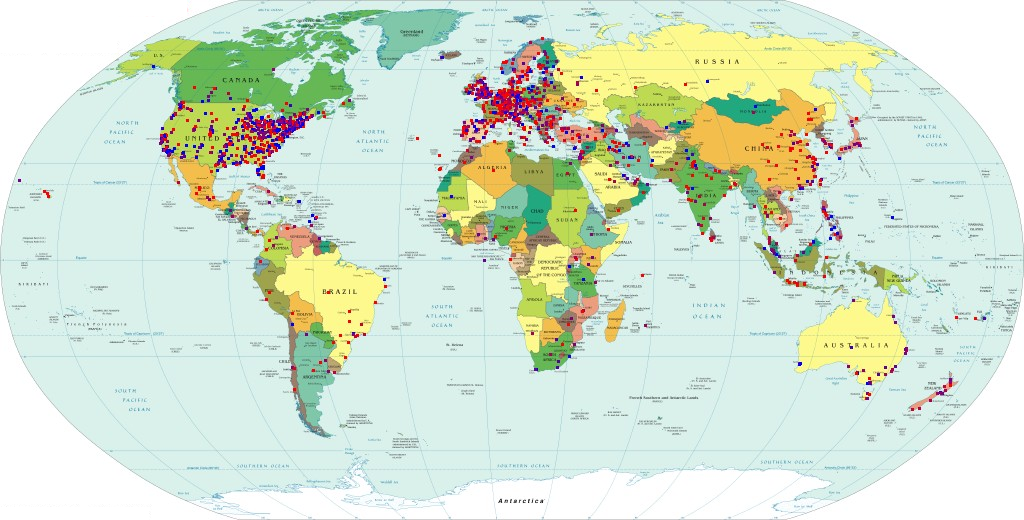
\includegraphics[width=\textwidth,keepaspectratio]{ImageGeneration-full}
	\caption{Sample output from the (single-layer) server-side image
		generation technique.}
	\label{fig-image}
\end{figure}


Single-layer techniques could use any of the distribution styles
discussed in Section~\ref{sec-distribution}. However, all but the image
server style would require the installation of additional client-side
software for generating images and performing cartographic projection
operations, so only single-layer techniques that use the image server
distribution style (or \textbf{server-side image generation} techniques)
are considered here. For this research, the author chose a
representative server-side image generation technique based on the GD
and PROJ.4 libraries.

Server-side image generation techniques provide some distinct
advantages. They are relatively simple to implement and are fast at
producing the final image, mainly because they use existing,
well-established technologies. They are also bandwidth efficient,
because the size of the generated map image is determined by its pixel
dimensions and the compression method used, rather than by the number of
points to be plotted. The amount of data to be sent to the client should
therefore remain more or less constant, regardless of the number of
points plotted.

Server-side image generation techniques also have some disadvantages,
however. First, a suitable base map image must be acquired. This could
be generated from a GIS, but if this is not an option an appropriate
image must be obtained from a third party. Care must be taken in the
latter case to avoid copyright issues. Second, the compression method
used to produce the final composite map image can have a significant
impact on visual quality. For example, lossy compression methods such as
JPEG can make the points plotted on the map appear distinctly fuzzy or
``muddy'', even at high quality levels. Lossless compression methods
such as PNG avoid this problem, but may produce larger files for the
same image. Finally, it is harder to provide interactive map
manipulation features with server-side image generation techniques, as
the output is a simple static image. Anything that changes the content
of the map (such as panning or changing the visibility of certain
points) will require the entire image to be regenerated. Zooming could
be achieved if a very high resolution base map image was available, but
the number of possible zoom levels is likely to be restricted.


\subsection{Multi-layer techniques}
\label{sec-overlay}

Multi-layer techniques also involve plotting points onto a base map
image, but they differ from single-layer techniques in that the points
are not plotted directly onto the base map image. Rather, the points are
displayed as an independent overlay on top of the base map image. This
provides a significant advantage over single-layer techniques, as it
enables the possibility of multiple independent layers that can be
individually shown or hidden. This is very similar to the multi-layer
functionality provided by a GIS, and is an effective way to provide
interactive visualizations of geographic data
\cite{Wood-J-1996-vis,MacE-AM-1998-GIS}. There is still the problem of
finding a suitable base map image, however.

Until relatively recently, implementing multi-layer techniques would
likely have required additional software to be installed at the client,
but most modern browsers now support absolute positioning of HTML elements
using CSS. This enables the creation of a map overlay using nothing more
than HTML, CSS and a few bitmap images. The author has identified two
main alternatives for producing such an overlay, which can be termed
\emph{image overlay} and \emph{HTML overlay}.

An image overlay comprises a transparent bitmap image into which the
points are plotted, which is then overlaid on the base map image (in the
author's implementation, the output looks essentially identical to that
shown in Figure~\ref{fig-image} on page~\pageref{fig-image}). This
requires the overlay image to be in either PNG or GIF format, as JPEG
does not support transparency. The overlay image is likely to contain
considerable ``white space'', which compresses very well, so use of a
lossless compression method should not be an issue. This also eliminates
the image quality issue noted earlier. The size of the image overlay
will generally be proportional to the number of points to be plotted,
but the image compression should moderate this.

As noted in Section~\ref{sec-image-gen}, generating images at the client
would require additional software to be installed, so only the data
server distribution style will be considered here for image overlays
(i.e., \textbf{server-side image overlay}). That is, both the base map
image and the overlay(s) are generated at the server.

An HTML overlay comprises a collection of HTML elements corresponding to
the points to be plotted, which are positioned over the base map image
using CSS absolute positioning. There is considerable flexibility as to
the types of elements that could be used to construct the overlay. One
possibility is to use \verb|<IMG>| elements to place icons on the base
map, which appears to be the approach adopted by Google Maps (see
Figure~\ref{fig-google}). Another possibility is to use appropriately
sized and colored \verb|<DIV>| elements, which then appear as colored
blocks ``floating'' over the base map image (in the author's
implementation, the output looks essentially identical to that shown in
Figure~\ref{fig-image} on page~\pageref{fig-image}).


\begin{figure}
	\centering
	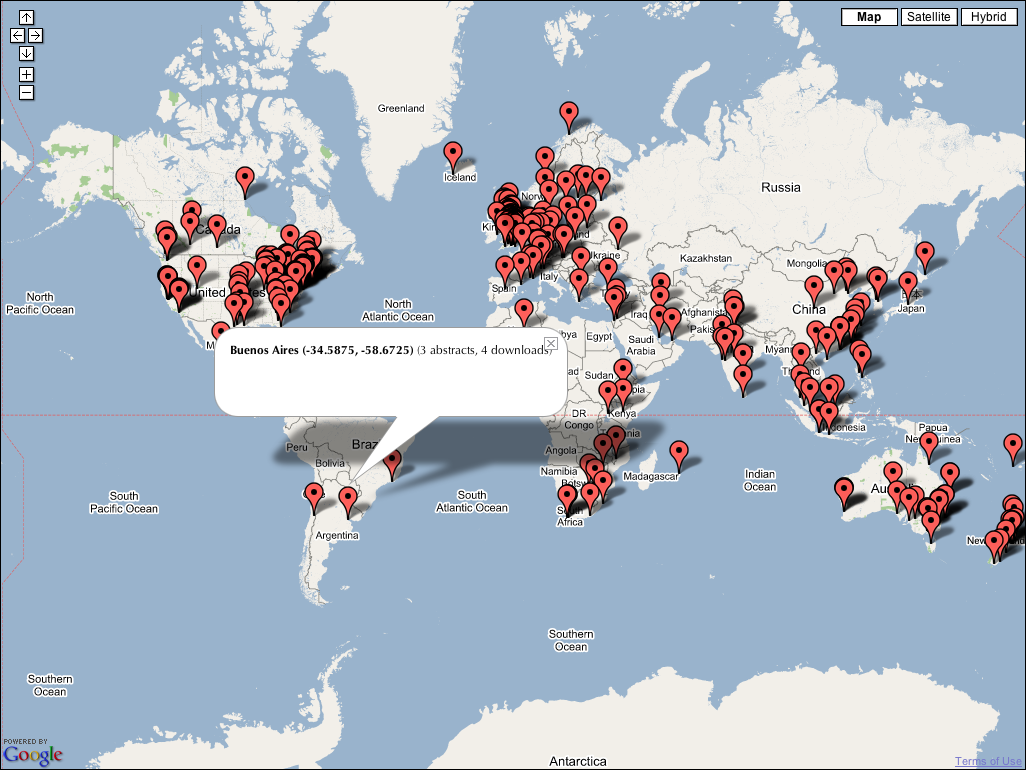
\includegraphics[width=\textwidth,keepaspectratio]{GoogleMap-full.png}
	\caption{Sample output from the (multi-layer) Google Maps technique.}
	\label{fig-google}
\end{figure}


HTML overlays may be generated at either the server or the client.
Unlike the techniques discussed previously, however, HTML overlays can
be generated at the client without the need for additional software,
because only HTML (i.e., text) is being generated, not images. This can
be easily achieved using client-side JavaScript, so HTML overlays can
use any of the distribution styles discussed in
Section~\ref{sec-distribution} without violating the requirement to
avoid additional client-side software. Two representative HTML overlay
techniques have thus been adopted for the experiments:
\textbf{server-side HTML overlays} (using the image server distribution
style) and \textbf{Google Maps} (using the data server distribution
style). Since Google Maps uses \verb|<IMG>| elements, \verb|<DIV>|
elements have been used for the server-side HTML overlay.

Server-side HTML overlays are actually slightly simpler to implement
than either server-side image generation or image overlays, because it
is not necessary to write any code to generate or manipulate images (the
base map image is static and thus requires no additional processing).
All that is required is code to transform latitude/longitude coordinates
into projected map coordinates and generate corresponding \verb|<DIV>|
elements.

Google Maps \cite{Goog-M-2006-maps} is a more complex proposition. This
technique uses the data server distribution style, where JavaScript code
running within the browser enables the client to manipulate the base map
and its overlays. Data and map images are requested asynchronously from
the server as required using Ajax technologies, which seems to imply
that Google Maps in fact uses the shared environment distribution style.
However, the server has no involvement beyond simply supplying data to
the client. In the shared environment distribution style, the server is
directly involved in manipulating the map, under the control of the
client. This is clearly not the case with Google Maps.

The primary advantage of Google Maps is the powerful and compelling
functionality it provides for generating and interacting with the map.
Users may pan the map in any direction and zoom to many different levels
of detail. A satellite imagery view is also available. In addition,
further information about each point plotted (such as the name of the
city) can be displayed in a callout attached to the point, as shown in
Figure~\ref{fig-google}. Google Maps also has a proven record for
visualization of network resources. For example,
\citeN{Gibb-H-2006-Gridscape} use Google Maps to visualize and manage
world-wide computing grids.

However, there are also some significant disadvantages to the Google
Maps technique\footnote{Interestingly, the Google Earth application
addresses many of these issues, but since it is not a browser-based
solution it falls outside the scope this research.}. First, it is a
distributed application, thus making it more complex to implement, test
and debug \cite{Bates-PC-1995-distdebug,Ensl-PH-1978-distributed}.
Second, the server must have a registered API key from Google, which is
verified every time that a page attempts to use the API. Similarly, the
client must connect to Google's servers in order to to download the
API's JavaScript source. This means that the technique requires an
active Internet connection in order to work. Finally, the Google Maps
API does not currently provide any way to toggle the visibility of
markers on the map, so it is not possible to implement the interactive
``layers'' mentioned at the start of this section. (It is possible, of
course, that Google may implement this feature in a future version of
the API.)

The most significant disadvantage of all HTML overlay techniques,
however, is that the size of the HTML overlay is directly proportional
to the number of points to be plotted. There will be one overlay element
(\verb|<DIV>| or \verb|<IMG>|) per point, so a very large number of
points will result in an even larger amount of HTML source being
generated. It is expected that this will lead to excessive browser
memory usage for large data sets, and consequently that these techniques
will not scale well at the high end. However, they may still be
appropriate for smaller data sets that require interactive manipulation.


\section{Experimental design}
\label{sec-experiment}

After some preliminary testing with live data from the Otago School of
Business repository, a series of experiments was undertaken to test the
scalability of the four chosen techniques. Each technique was tested
using the same collection of progressively larger synthetic data sets.
The first data set comprised one point at the South Pole. A regular grid
of points at one degree intervals was then constructed by progressively
incrementing the latitude and longitude, with each data set being twice
the size of its predecessor. A total of twenty-one data sets were
created in this way, with the number of points ranging from one to
1,048,576 (\(=2^{20}\)). The result of plotting the 16,384-point data
set is shown in Figure~\ref{fig-grid-points}. The grid spacing used
meant that 64,800 points were sufficient to fill the entire map, so the
five largest data sets had many duplicate points. This does not affect
the results of the experiments, however, as it is the total number of
points that is significant, not their location.


\begin{figure}
	\centering
	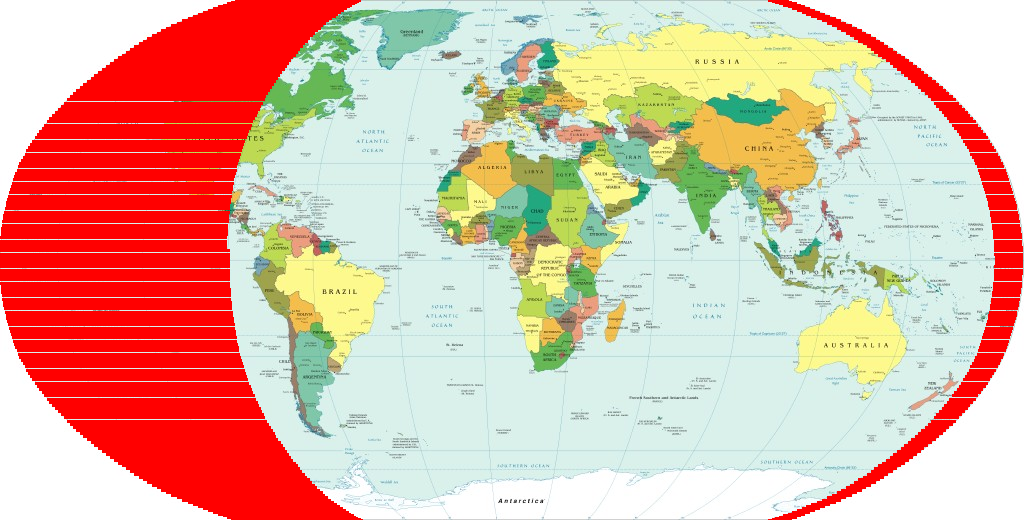
\includegraphics[width=\textwidth,keepaspectratio]{16384_points}
	\caption{The 16,384-point data set plotted on the base map.}
	\label{fig-grid-points}
\end{figure}


The focus on scalability meant that the primary measures of interest
were page load time, memory usage and the volume of data generated
(which impacts on both storage and network bandwidth). Page load time
can be further broken down into the time taken to generate the map data,
the time taken to transfer the map data and other ancillary material to
the client across the network, and the time taken by the client to
display the map.

Unfortunately, as noted in Section~\ref{sec-overlay}, the Google Maps
technique requires an active Internet connection, so the experiments
could not be run on an isolated network. This meant that traffic on the
local network was a potential confounding factor. It was therefore
decided to eliminate network performance from the equation by running
both the server and the client on the same machine\footnote{A Power
Macintosh G5 1.8\,GHz (single processor) with 1\,GB RAM, running Mac OS
X 10.4.7, Apache 2.0.55, PHP 4.4 and Perl 5.8.6.}. This in turn enabled
independent measurement of the times for data generation and page
display, thus simplifying the process of data collection and also
ensuring that the client and server processes did not unduly interfere
with each other, despite running on the same machine.

It could be argued that network performance would still have a
confounding effect on the Google Maps technique, but this would only be
likely for the initial download of the API (comprising about 235\,kB of
JavaScript source and images), which would be locally cached thereafter.
The API key verification does occur every time a map is loaded, but
the amount of data involved is very small, so it is less likely that
this would be significantly affected by network performance. Any such
effect would also be immediately obvious as it would simply block the
server from proceeding.

For each data set generated, its size, the time taken to generate it,
the time taken to display the resultant map in the browser, and the
amount of real and virtual memory used by the browser during the test
were recorded. It was also intended to measure the memory usage of the
server, but this proved more difficult to isolate than expected, and was
thus dropped from the experiments. The data set generation time and
browser memory usage were measured using the \texttt{time} and
\texttt{top} utilities respectively (the latter was run after each test
run to avoid interference). The map display time was measured using the
``page load test'' debugging feature of Apple's Safari web browser,
which can repetitively load a set of pages while recording various
statistics, in particular the time taken to load the page. Tests were
run up to twenty times each where feasible, in order to reduce the
impact of random variations. Some tests were run fewer times because
they took an excessive amount of time to complete. Further testing for a
particular technique was generally halted when a single test run took
longer than about five minutes, as by this stage performance had already
deteriorated well beyond usable levels. The web browser was quit and
reloaded afresh before each group of tests.


\subsection{Technique implementation}

As noted in Sections~\ref{sec-image-gen} and \ref{sec-overlay}, the
server-side image generation, server-side image overlay and server-side
HTML overlay techniques were all implemented using the image server
distribution style. A separate dispatcher page was written in PHP for
each technique, which enabled arguments---such as the number of points
to be plotted---to be passed from the client to a corresponding Perl
script for each technique. The final page was then constructed as
follows:
\begin{description}

	\item[server-side image generation] The dispatcher page included a
	standard \verb|<IMG>| element that called the Perl script. This
	script loaded a base map PNG image, plotted points directly onto it,
	and returned the composite map to the client as a JPEG image (with
	the ``quality'' parameter set to 90).

	\item[server-side image overlay] The dispatcher page included two
	\verb|<IMG>| elements, the first for the base map and the second for
	the overlay, both with identical CSS positioning attributes. The
	first \verb|<IMG>| simply loaded a static JPEG image representing
	the base map. The second \verb|<IMG>| called the Perl script, which
	generated and returned the overlay as a transparent PNG image.

	\item[server-side HTML overlay] The dispatcher page included an
	\verb|<IMG>| element for the base map and a \verb|<DIV>| element for
	the overlay, both with identical CSS positioning attributes. The
	\verb|<IMG>| simply loaded a static JPEG image representing the base
	map. The \verb|<DIV>| contained inline PHP code that called the Perl
	script. This in turn generated and returned the overlay as a
	collection of CSS-positioned \verb|<DIV>| elements, nested within
	the top-level \verb|<DIV>| element.

\end{description}

For all of these techniques, the base map image was 1,024 \(\times\) 520
pixels. In PNG format it occupied approximately 1.2\,MB (but this
version was never returned to the client), while in JPEG format (Q=90)
it occupied approximately 180\,kB. The base map image was derived from
an original 3,599 \(\times\) 1,826 pixel image, which was part of a
collection of maps released into the public domain by the
\citeN{CIA-WFB-2006}. All three techniques used the PROJ.4 cartographic
projections library to convert latitude/longitude pairs into projected
map coordinates, while the first two techniques also used the GD
graphics library to programmatically generate and manipulate images.

The Google Maps technique was implemented using the data server
distribution style. As with the other three techniques, a PHP dispatcher
page was used. This time, however, the page included client-side
JavaScript code to load and initialize the Google Maps API, create the
base map, and build the map overlay. The first two steps were achieved
using standard Google Maps API calls. For the last step, the client used
an \texttt{XMLHttpRequest} object to asynchronously call a server-side
Perl script, which generated and returned to the client an XML data set
containing the points to be plotted. The client then looped through this
data set and used Google Maps API calls to create a marker on the base
map corresponding to each point.


\section{Results}
\label{sec-results}

As noted in the introduction, the intent of these experiments was not to
do a full analysis and statistical comparison of the performance of the
different techniques, but rather to identify broad trends. There has
not, therefore, been any statistical analysis carried out on the
results. The remainder of this section will discuss the results for data
size, page load time and memory usage. Because the number of points in
each data set increases in powers of two, log-log scales have been used
for all plots.


\subsection{Data size}

For each data set, the data generated by the server was saved to a file
and its size in bytes recorded. In the case of the server-side image
generation and server-side image overlay techniques, the file comprised
a bitmap image; whereas for the server-side HTML overlay and Google Maps
techniques, the file comprised HTML or XML text, respectively.

In addition to the generated data, there was a certain amount of fixed
overhead associated with each technique tested, as summarized in
Table~\ref{tab-overhead}. This overhead comprised static files that were
always downloaded to the client regardless of the number of points to be
plotted. Examples of fixed overhead items include the base map image,
various icons, the PHP source of the dispatcher page and the JavaScript
source for the Google Maps API.


\begin{acmtable}{11cm}
	\centering
	\begin{tabular}{lll}
		Technique						&	Fixed overhead		&	Content	\\
		\hline
		Server-side image generation	&	629\,bytes			&	\textbf{dispatcher (PHP)}\medskip	\\

		Server-side image overlay		&	\(\approx\) 181\,kB	&	dispatcher (PHP) \\
										&						&	\textbf{base map image (JPEG)}\medskip	\\

		Server-side HTML overlay		&	\(\approx\) 181\,kB	&	dispatcher (PHP) \\
										&						&	\textbf{base map image (JPEG)}\medskip	\\

		Google Maps						&	\(\approx\) 235\,kB	&	dispatcher (PHP) \\
										&						&	base map image tiles (PNG) \\
										&						&	\textbf{API (JavaScript)} \\
										&						&	various icons (PNG)	\\
	\end{tabular}
	\caption{Fixed overhead for each technique. The largest contributing
	item for each technique is shown in \textbf{bold face}.}
	\label{tab-overhead}
\end{acmtable}


\begin{figure}
	\centering
	\includegraphics[scale=0.55]{data_size}
	\caption{Comparison of generated data size for each technique (log-log scale).}
	\label{fig-data-size}
\end{figure}


The volume of data generated by each technique, including fixed
overhead, is shown in Figure~\ref{fig-data-size}. It is immediately
apparent from these results that there is a divergence between the two
techniques that generate images (server-side image generation and
server-side image overlay), and the two techniques that generate text
(server-side HTML overlay and Google Maps).

Both the server-side image generation and server-side image overlay
techniques scale particularly well with regard to the amount of data
generated. Interestingly, the amount of data generated by the image
generation technique increases by about 8\,kB up to the 8,192-point data
set, but then \emph{drops} by about 90\,kB over the next three data
sets. This occurs because the number of points plotted has become
sufficient to cover most of the base map. This means that a large
portion of the composite map image is a single color (see
Figure~\ref{fig-grid-points} on page~\pageref{fig-grid-points} for an
example), which compresses more efficiently.

The amount of data generated by the image overlay technique appears
constant, but actually increases by about 2\,kB across the range. This
has important implications for the ability of this technique to handle
multiple layers. Because the overlay images are quite small (less than
2\,kB for up to one million points), it should be feasible to pre-load
several overlay images into a client-side array and switch them on and
off as desired.

The server-side HTML overlay and Google Maps techniques clearly do not
scale well with respect to data size, and begin to visibly diverge from
the other two techniques once the amount of data generated exceeds about
5\% of the fixed overhead. For the HTML overlay technique this occurs
somewhere between 64 and 128 points, whereas for Google Maps it occurs
somewhere between 256 and 512 points. The divergence increases rapidly
for both techniques beyond these points, with the HTML overlay technique
suffering the most. The latter occurs because the HTML overlay technique
needs to generate additional CSS attributes (i.e., more text) in order
to correctly position the \verb|<DIV>| elements, whereas the Google Maps
technique needs only to return a more compact list of latitude/longitude
coordinates.


\subsection{Page load time}

For each test run, both the length of time taken to generate the data at
the server and to display the page in the client browser were recorded.
The former is illustrated in Figure~\ref{fig-data-generation-time} and
the latter in Figure~\ref{fig-page-load-time}. The combined time (data
generation + display time) is shown in Figure~\ref{fig-combined-time}.


\subsubsection{Data generation time}


\begin{figure}
	\centering
	\includegraphics[scale=0.55]{data_generation_time}
	\caption{Comparison of data generation time for each technique (log-log scale).}
	\label{fig-data-generation-time}
\end{figure}


The results (see Figure~\ref{fig-data-generation-time}) show that the
length of time taken to generate the source data increases in proportion
to the number of points to be plotted, as expected. It is interesting to
note the differences in data generation time for each technique,
however. Data generation for both of the ``text-based'' techniques (HTML
overlay and Google Maps) is generally faster than for the
``image-based'' techniques (image generation and image overlay).

The results show that server-side image generation generally takes the
longest to generate its data. This is because it not only has to map
points from latitude/longitude into projected map coordinates, but also
must plot these points onto the base map image, then compress the
composite image as a JPEG. The image to be compressed is also moderately
complex, which only adds to the data generation time. Server-side image
overlay performs somewhat better because it uses a less complex
compression method (PNG) and the image to be compressed is much simpler
(a collection of colored points on a blank background).

The server-side HTML overlay technique appears faster at generating data
than either of the two image-based techniques at the low end, but is
similar in performance at the high end. In this technique the server
only needs to map latitude/longitude to projected map coordinates; no
images need to be generated and there is no compression to deal with. At
the high end, however, this advantage is clearly offset by the
significant volume of data being generated. Google Maps is faster again,
because almost all processing is carried out on the client; the server's
only involvement is to generate a simple list of latitude/longitude
coordinates.

In terms of data generation, it appears that all techniques tested scale
reasonably well. The image-based techniques perform worse at the low end
because they involve more complex processing than the text-based
techniques, but this is offset at the high end by the relatively
constant amount of data generated. Conversely, the text-based techniques
perform better at the low end, but are negatively impacted at the high
end by the sheer volume of data produced (tens or hundreds of megabytes
vs.\ hundreds of kilobytes).


\subsubsection{Map display time}


\begin{figure}
	\centering
	\includegraphics[scale=0.55]{page_load_time}
	\caption{Comparison of map display time for each technique (log-log scale).}
	\label{fig-page-load-time}
\end{figure}


These results (see Figure~\ref{fig-page-load-time}) reveal quite a
spectacular difference between the image-based and text-based
techniques. The time taken to display the map is essentially constant
for both of the image-based techniques, regardless of the number of
points to be plotted. This is not surprising given that the size of the
generated data is also essentially constant, and that the browser is
simply loading and displaying static images. The image overlay technique
appears slightly slower than the image generation technique. This is
probably because the image overlay technique has to load two images from
the server (the base map and the overlay), compared to one image for the
image generation technique.

In contrast, the text-based techniques clearly do not scale well with
respect to map display time. Google Maps suffers particularly in this
regard, with display time exceeding ten seconds shortly past 512 points.
Testing was abandoned at 4,096 points, with a single test run taking
over seven minutes. The HTML overlay technique fares better, exceeding
ten seconds somewhere between 4,096 and 8,192 points. Testing was
abandoned at 32,768 points, with a single test run taking almost ten
minutes.


\subsubsection{Combined time}


\begin{figure}
	\centering
	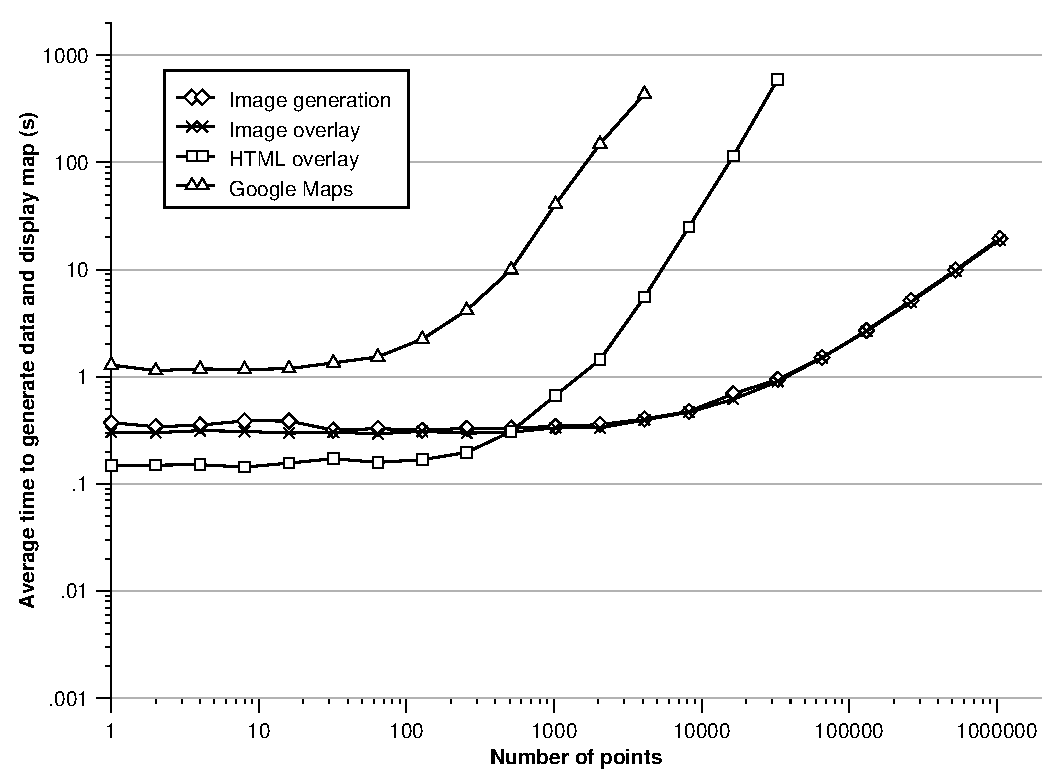
\includegraphics[scale=0.55]{combined_time}
	\caption{Comparison of combined page load time for each technique (log-log scale).}
	\label{fig-combined-time}
\end{figure}


Combining the data generation and map display times (see
Figure~\ref{fig-combined-time}) yields little change in the curves for
the text-based techniques, because the data generation times are very
small compared to the map display times. There is a more obvious impact
on the image-based techniques, with both techniques remaining more or
less constant up to about 2,048 points, then slowing as the number of
points increases beyond that. However, the slowdown is nowhere near as
dramatic as for the text-based techniques; even the largest data set
only takes about nineteen seconds overall. The image overlay technique
does display a slight advantage of about half a second over the image
generation technique for the largest data set, but further experiments
will be required to determine whether this difference is statistically
significant.


\subsection{Memory usage}

Both the real and virtual memory usage of the browser were measured by
running the \texttt{top} utility after each test run and observing the
memory usage in each category. This provided the size of both the
current ``working set'' and the total memory footprint of the browser
process after it had completed a test run. The real memory results are
shown in Figure~\ref{fig-real-memory} and the virtual memory results are
shown in Figure~\ref{fig-virtual-memory}.


\begin{figure}
	\centering
	\includegraphics[scale=0.55]{real_memory}
	\caption{Comparison of browser real memory usage for each technique
	(log-log scale).}
	\label{fig-real-memory}
\end{figure}


\begin{figure}
	\centering
	\includegraphics[scale=0.55]{virtual_memory}
	\caption{Comparison of browser virtual memory usage for each
	technique (log-log scale).}
	\label{fig-virtual-memory}
\end{figure}


While both sets of results display similar trends, the real memory data
proved somewhat problematic. Real memory usage was generally consistent
across test runs, but would also frequently fluctuate upwards by a
factor of nearly two for no readily apparent reason. This is
particularly apparent with the HTML overlay technique beyond 1,024
points. It seems likely that this was a result of other processes on the
test machine interacting with the browser process in unexpected ways.
There is some doubt therefore as to the validity of the real memory
data, but they are at least broadly consistent with the virtual memory
data. The virtual memory data proved more consistent overall, as the
virtual memory footprint of a process is less likely to be impacted by
other running processes.

The results show that the two image-based techniques have essentially
constant virtual memory usage of about 170\,MB regardless of the number
of points plotted. This is to be expected, given that the size of the
generated data is also essentially constant. The text-based techniques,
however, clearly begin to diverge as the number of points increases. The
HTML overlay technique starts to visibly diverge somewhere between 2,048
and 4,096 points, reaching a maximum of about 216\,MB at the point that
testing was terminated. Google Maps starts to visibly diverge between 64
and 128 points, reaching a maximum of about 264\,MB at the point that
testing was terminated. This is in line with the initial expectation for
these techniques, that is, that memory usage would increase in
proportion to the number of points to be plotted.


\section{Conclusion and future work}
\label{sec-conclusion}

In this research, the scalability of four techniques for
online geovisualization of web site hits was tested, with respect to the number of
points to be plotted on the map. The four techniques tested were
server-side image generation, server-side image overlay, server-side
HTML overlay and Google Maps. The results clearly show that the
server-side image generation and server-side image overlay techniques
scale the best from small to large data sets. The HTML overlay and
Google Maps techniques work well for small data sets, but their
performance rapidly deteriorates as the size of the data set increases,
to the point where they become unusable.

Despite this clear difference in scalability, there are still some
interesting questions remaining. The model interaction environment
distribution style was not investigated in this research, as it was
unclear whether this could be achieved using only client-side
JavaScript. This is clearly an avenue for further investigation. In
addition, the appearance of native SVG support in browsers means that
this may become a viable option for implementing this distribution style
in future.

It was somewhat surprising that the server-side HTML overlay and Google
Maps techniques exhibited no obvious consistency in where the different
measures (data size, map display time and virtual memory usage)
diverged, as shown in Table~\ref{tab-divergence}. Google Maps appears to
exhibit greater consistency than HTML overlay in this respect, but it
seems logical to expect some form of correlation, so further research
will be required to investigate this. One possibility might be to
implement an instrumented web browser and server in order to gather more
precise data.


\begin{acmtable}{11cm}
	\centering
	\begin{tabular}{lccc}
		Technique						&	Data size	&	Map display time	&	Virtual memory	\\
		\hline
		Server-side HTML overlay		&	64--128		&	128--256			&	2,048--4,096 \\
		Google Maps						&	256--512	&	64--128				&	64--128	\\
	\end{tabular}
	\caption{Approximate number of points at which each measure begins to
		visibly diverge, for the HTML overlay and Google Maps techniques.}
	\label{tab-divergence}
\end{acmtable}


Shortly after completing the experiments, the author discovered
\emph{msCross Web\-gis}\footnote{\url{http://datacrossing.crs4.it/en_Documentation_mscross.html}},
an open source Google Maps clone. Its documentation implies that it may
be possible to build a fully self-contained implementation that requires
no external network access. This would enable testing on an isolated
network with the client and server running on different machines.
Measurements of network transfer time could then be included, and any
issues arising from running the client and server on the same machine
would be eliminated. This would require a distributed measurement
infrastructure similar to that developed by \citeN{Barf-P-1999-webperf}.

The overall aim of this work was to identify the best technique for
plotting the large number of downloads and abstract views from the Otago
School of Business digital repository. Based on the results, both the
server-side HTML overlay and Google Maps techniques are clearly
inappropriate for this task. This leaves a choice between two very
similarly-performing techniques: server-side image generation and
server-side image overlay. However, multi-layer techniques display many
practical advantages over single-layer techniques, such as the ability
to dynamically show and hide multiple overlays. These advantages provide
greater flexibility and a more dynamic experience for end-users. Taking
these end-user benefits into consideration, the server-side image
overlay technique is the clear winner in this case.


\begin{acks}
The author would like to acknowledge Dr.\ Antoni Moore and Prof.\ George
Benwell for their input into this research.
\end{acks}


\bibliography{Map_Visualisation}


\begin{received}
...
\end{received}
\end{document}


